\chapter{Sviluppo del software di analisi}
La realizzazione di un software dedicato all'analisi dei dati bibliometrici è al centro di questo capitolo. Attraverso una combinazione di tecnologie, il software mira a fornire agli utenti gli strumenti necessari per esplorare, analizzare e visualizzare le analisi sui fattori bibliometrici degli autori di paper scientifici.
Nel corso di questo capitolo verrà esplorata l'architettura del software, gli strumenti e le tecnologie utilizzate, le analisi e i grafici implementati.

\section{Architettura client/server}
Le esigenze di analisi complesse, la necessità di una visualizzazione chiara e interattiva dei dati e l'importanza di condividere facilmente gli output con altri utenti hanno reso imperativo l'adozione di un'architettura robusta e flessibile per il software di analisi dei dati, l'architettura client/server si è rivelata la scelta ideale per soddisfare queste esigenze.

Nel presente contesto, il server svolge un ruolo cruciale nell'elaborazione delle richieste, eseguendo analisi dettagliate e restituendo i risultati pertinenti al client. Gestisce anche in modo efficiente l'interazione con il database MongoDB e mette a disposizione un servizio API RESTful, facilitando l'accesso e la manipolazione dei dati. Parallelamente, il client invia richieste specifiche al backend per ottenere o eseguire determinate analisi e, una volta ricevute, presenta i risultati attraverso un'interfaccia utente interattiva, garantendo che gli utenti possano comprendere e interpretare le informazioni in modo chiaro e intuitivo.

\section{Strumenti e tecnologie utilizzate}
Nel processo di sviluppo del software, particolare attenzione è stata posta nella scelta delle tecnologie e degli strumenti. Per il componente di backend la scelta del linguaggio Python è stata naturale considerando sia la volontà di mantenere una coerenza con il modulo di download e aggregazione dei dati descritto nel Capitolo~\ref{scopusBulkDownloader}, sia la sua vasta gamma di librerie dedicate all'analisi dei dati. Per accelerare lo sviluppo e garantire un'implementazione solida dell'infrastruttura web, è stato adottato Flask \cite{flask-github}, un micro framework web noto per la sua semplicità e efficienza.

Per il frontend, invece, la scelta è ricaduta su TypeScript \cite{typescript}, un linguaggio open source che estende JavaScript introducendo la tipizzazione statica. La decisione di utilizzare React \cite{react-github} come libreria per la costruzione delle interfacce utente è stata guidata dalla sua capacità di offrire un'esperienza utente fluida e reattiva, oltre alla sua popolarità e alla vasta comunità di supporto. Un'altra libreria utilizzata di fondamentale importanza è Apache ECharts \cite{apache-echarts-github}, una soluzione open source dedicata alla visualizzazione dei dati, sviluppata per creare grafici e diagrammi interattivi per il web mantenuta da Apache Software Foundation.

All'interno del lavoro sono state integrate altre librerie per semplificare lo sviluppo e potenziare le funzionalità del software, tra queste c'è Mui \cite{mui-github}, un framework UI per React basato sul Material Design \cite{material-design} di Google che ha giocato un ruolo chiave nella realizzazione di un'interfaccia grafica intuitiva e reattiva. Sul lato backend, Pandas e PyMongo sono stati essenziali per l'elaborazione, l'analisi e la gestione dei dati, queste librerie sono già state approfondite nel Paragrafo~\ref{scopusBulkDownloader-tech}.

Data la complessità e l'eterogeneità delle tecnologie impiegate in questo progetto, l'adozione di Docker \cite{docker} è stata una scelta strategica per garantire una gestione fluida e centralizzata delle numerose dipendenze. L'uso dei container ha permesso di incapsulare ogni componente del sistema in ambienti isolati, facilitando così non solo l'installazione, ma anche l'aggiornamento e la manutenzione, assicurando che ogni parte del software operi in condizioni ottimali e coerenti. Questo approccio ha inoltre contribuito a rendere il sistema più robusto e resiliente, minimizzando i rischi legati a possibili incompatibilità o conflitti tra le diverse librerie e servizi utilizzati.


\section{Funzionalità di analisi dei dati}
Il backend del progetto implementa sei diverse funzionalità di analisi dei dati, che sono:
\begin{enumerate}
    \item \textbf{Variazione media dei coautori nel tempo}: questa funzione calcola come varia il numero medio di coautori negli anni successivi all'inizio della carriera di un autore, considerando autori con un $h$-index superiore a una certa soglia decisa dall'utente.

    \item \textbf{Impatto del numero di coautori sulle citazioni}: valuta la relazione tra il numero di coautori di un articolo e il numero di citazioni che quest'ultimo ha ricevuto.

    \item \textbf{Analisi del momento di pubblicazione di articoli influenti sull'$h$-index}: definisce in quale momento della carriera di un autore sono stati pubblicati gli articoli che influenzano l'$h$-index normalizzando il risultato tra 0 (inizio carriera) e 1 (fine carriera). Nel Codice~\ref{lst:analyze_hindex_influential_articles_timing} vi è la porzione che illustra il processo di calcolo del momento di pubblicazione e relativa normalizzazione.
    Considera esclusivamente autori con un $h$-index superiore a una certa soglia decisa dall'utente.

    \item \textbf{Correlazione tra $h$-index e articoli esclusi}: cerca una correlazione tra il valore di $h$-index di un autore e il numero di articoli che non sono considerati nel calcolo di quest'indice, considerando esclusivamente autori con un $h$-index superiore a una certa soglia decisa dall'utente.

    \item \textbf{Correlazione tra $h$-index e durata della carriera}: esplora la relazione tra l'$h$-index di un autore e la durata della sua carriera.

    \item \textbf{Impatto del ranking di una conferenza sul numero di citazioni}: esamina se esiste una correlazione tra il numero di citazioni ricevute da un articolo e il ranking della conferenza in cui è stato presentato, considera esclusivamente autori con un $h$-index superiore a una certa soglia decisa dall'utente.

\end{enumerate}

\begin{lstfloat}
    \begin{lstlisting}[
    language=Python,
    caption={Calcolo del momento di pubblicazione e normalizzazione},
    label={lst:analyze_hindex_influential_articles_timing},
    breaklines=true,
    postbreak=\mbox{\textcolor{red}{$\hookrightarrow$}\space}
    ]
df_abstracts = df_abstracts \
    .sort_values('citedby_count', ascending=False) \
    .head(h_index)

df_abstracts['years_since_career_start'] = pd \
    .to_datetime(df_abstracts['coverDate']) \
    .dt.year - career_start_year

max_difference = career_end_year - career_start_year

df_abstracts['coefficient'] = \
    df_abstracts['years_since_career_start'] / max_difference
    
return df_abstracts['coefficient'].mean()
    \end{lstlisting}
\end{lstfloat}

Ognuna delle analisi sopra descritte è accessibile tramite specifici endpoint API RESTful, descritti in Tabella~\ref{table:api_endpoints}, progettati per fornire al client risposte in formato JSON, facilitando così la richiesta e la rappresentazione dei risultati.

\begin{table}[ht]
    \centering
    \begin{tabularx}{\textwidth}{|X|l|l|}
        \hline
        \textbf{Endpoint} & \textbf{Parametri} & \textbf{Valore default} \\
        \hline
        \url{/api/saved\_analyses} & - & - \\
        \hline
        \url{/api/all\_analyses} & \texttt{h-index}, \texttt{title} & 0, ``\texttt{analysis-0-hindex}'' \\
        \hline
        \url{/api/average\_coauthors\_variation\_after\_years} & \texttt{h-index} & 0 \\
        \hline
        \url{/api/coauthors\_impact\_on\_citations\_and\_hindex} & - & - \\
        \hline
        \url{/api/analyze\_hindex\_influential\_articles\_timing} & \texttt{h-index} & 0 \\
        \hline
        \url{/api/correlation\_between\_hindex\_and\_excluded\_articles} & \texttt{h-index} & 0 \\
        \hline
        \url{/api/correlation_between_hindex_and_career_duration} & - & - \\
        \hline
        \url{/api/citation\_count\_based\_on\_conference\_ranking} & \texttt{h-index} & 0 \\
        \hline
    \end{tabularx}
    \caption{Elenco degli endpoint API RESTful}
    \label{table:api_endpoints}
\end{table}

La struttura della risposta ha un campo principale contenente il risultato scalare dell'analisi e un campo \texttt{data} contenente una lista di valori o di coppie di dati utilizzati per il calcolo del campo principale; nel Codice~\ref{lst:example_json_response} è riportato un esempio di risposta.

\begin{lstfloat}
    \begin{lstlisting}[
    basicstyle=\ttfamily,
    caption={Esempio di risposta JSON di un'analisi},
    label={lst:example_json_response},
    ]
{
    "correlation": -0.06749014708602911,
    "data": [
        {
            "years_since_career_start": 0,
            "coauthors_count": 3.25
        },
        {
            "years_since_career_start": 1, 
            "coauthors_count": 4.6470588235
        },
        {
            "years_since_career_start": 2,
            "coauthors_count": 2.25
        },
        ...
    ]
}
    \end{lstlisting}
\end{lstfloat}

Quando viene invocata la funzione dell'endpoint \texttt{all\_analyses}, il sistema salva automaticamente i risultati delle analisi in una collezione MongoDB chiamata ``cacheAnalysis'' identificandoli tramite un nome e il valore di $h$-index scelto. Questa metodologia permette di accedere e visualizzare le elaborazioni passate in modo veloce e efficiente, eliminando la necessità di riprocessare i dati ad ogni nuova interrogazione.

\section{Dashboard}
Per facilitare la visualizzazione e la manipolazione dei dati analitici, è stata sviluppata una dashboard articolata in due sezioni principali. La prima offre agli utenti la possibilità di consultare e scaricare le interrogazioni precedenti, nonché di iniziare nuove analisi inserendo parametri specifici come il nome e l'$h$-index di soglia minima. La seconda sezione, invece, è dedicata alla rappresentazione dei risultati attraverso l'impiego di grafici. La Figura~\ref{fig:dashboard} illustra l'aspetto finale di questa interfaccia.

\begin{figure}[ht]
    \centering
    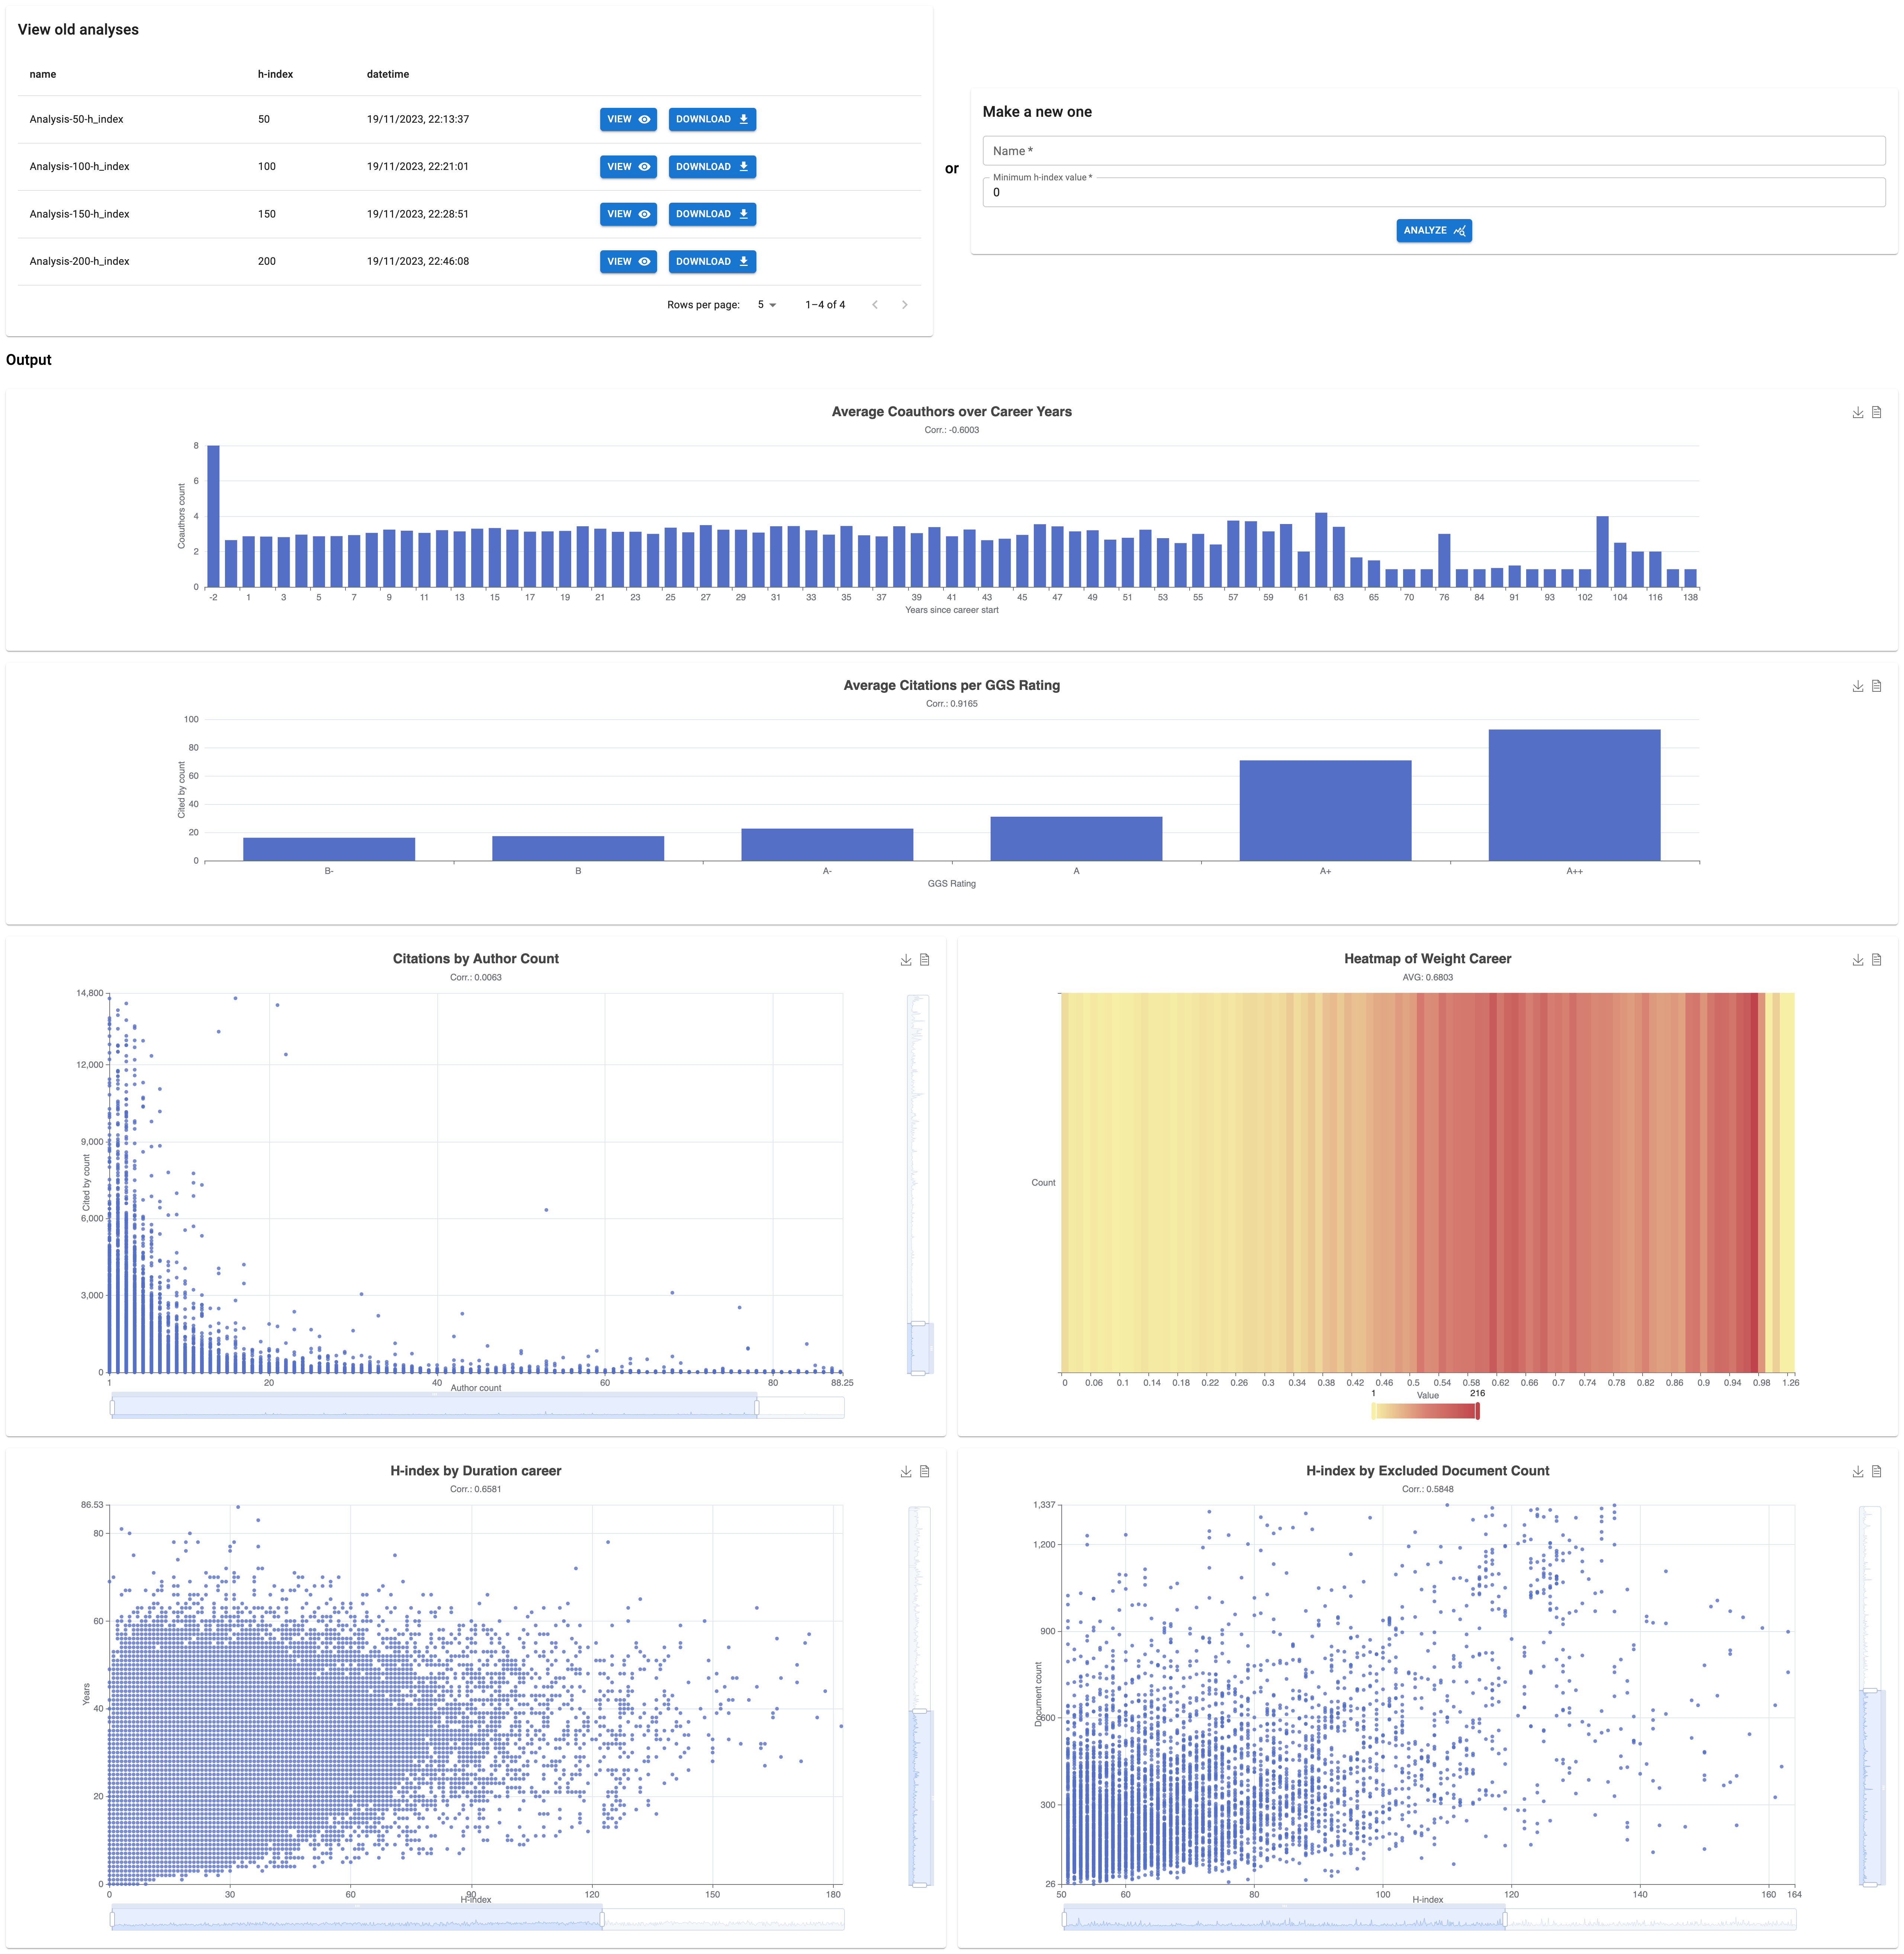
\includegraphics[width=0.9\textwidth]{images/dashboard.png}
    \caption{Dashboard}
    \label{fig:dashboard}
\end{figure}


I diagrammi sono stati accuratamente selezionati per adattarsi alle diverse nature dei dati: i grafici di dispersione offrono una visione dinamica delle variazioni e delle tendenze, i grafici a barre permettono un confronto immediato tra diverse categorie, e le mappe di calore espongono le relazioni complesse attraverso una gradazione cromatica. 
Ogni diagramma è scaricabile in formato vettoriale assicurando che la qualità delle immagini rimanga inalterata a prescindere dallo scaling, permettendo così una visualizzazione ottimale in ogni contesto, sia esso digitale o cartaceo.
Inoltre per i grafici a dispersione è stata aggiunta la possibilità di ingrandire determinate aree per visualizzare meglio zone con alte concentrazioni di dati.

Per completare l'offerta di strumenti a disposizione degli utenti, è stata introdotta una funzionalità di esportazione che permette di scaricare sia i dati delle analisi che i grafici corrispondenti in formato vettoriale, raccolti in un unico file .zip. Questo aspetto facilita notevolmente la distribuzione e la condivisione dei risultati, rendendo il processo di esportazione un'operazione semplice e veloce. La creazione dell'archivio compresso è resa possibile dall'impiego della libreria JSZip \cite{jszip}, come illustrato nel Codice~\ref{lst:export_archive_ts}.

\begin{lstfloat}
    \begin{lstlisting}[
    language=JavaScript,
    caption={Esportazioni dati e immagini},
    label={lst:export_archive_ts},
    breaklines=true,
    postbreak=\mbox{\textcolor{red}{$\hookrightarrow$}\space}
    ]
const exportData = (data: Analysis) => {
    const zip = new JSZip();
    const analysis = zip.folder('analysis');
    getAllEcharts()
    .forEach((instance: ECharts, index: number) => {
        let dataUrl = decodeURIComponent(instance.getDataURL());
        dataUrl = dataUrl.substring(dataUrl.indexOf(',') + 1);
        analysis?.file(`chart-${index}.svg`, dataUrl);
    });
    
    analysis?.file(
      `${data.name}.json`, 
      JSON.stringify(data)
    );
    
    zip.generateAsync({type:'blob'})
    .then(function(content) {
      saveAs(content, `${data.name}.zip`);
    });
};
    \end{lstlisting}
\end{lstfloat}

